\documentclass{article}
\usepackage[spanish]{babel}
% \usepackage[utf8]{inputenc}
\usepackage{graphicx}
\usepackage{amsmath}
\usepackage{geometry}
\usepackage{caption}
\usepackage{url}
\geometry{margin=1in}

\title{Primer Examen Parcial - Visión Computacional}
\author{
  \begin{minipage}[t]{0.4\linewidth}
    \centering
    Quistian Navarro, Juan Luis\\
    A341807@alumnos.uaslp.mx 
  \end{minipage}
}
\date{\today}

\begin{document}

\maketitle
\section{Planteamiento del problema}
Se cuenta con la imagen \texttt{"Jorge\_Campos.jpg"}, que ha sido editada para contener ruido que genera un efecto de desenfoque. El objetivo es aplicar una serie de filtros y operaciones proveniente de OpenCV \cite{opencvimgprocfilter} para eliminar el ruido, mejorar la nitidez y rotar la imagen de manera que la silueta de la persona aparezca completamente vertical. Además, se debe recortar la imagen para que solo aparezca la silueta de la persona lo más ceñido posible.

\section{Descripción de la solución}
El proceso de solución se basa en la aplicación de varios filtros de convolución y Fourier para eliminar el ruido y mejorar la calidad de la imagen. A continuación se detallan los pasos aplicados en el orden correspondiente:

\subsection{Filtro Sharpened (Convolución)}
El primer filtro aplicado fue un filtro de convolución Sharpened para mejorar la nitidez de los bordes y recuperar detalles de la imagen. Utilizamos un kernel Laplaciano con la función \texttt{cv2.filter2D()} de OpenCV.

\textbf{Kernel aplicado}:
\[
    \begin{bmatrix}
        -1 & -1 & -1 \\
        -1 & 9  & -1 \\
        -1 & -1 & -1
    \end{bmatrix}
\]

Este kernel tiene el efecto de resaltar los bordes y contrastar las áreas circundantes para mejorar la claridad de la imagen.

\subsection{Filtro Non-local Means}
El siguiente filtro aplicado fue el \texttt{Non-local Means} \cite{opencv_non_local_means}, el cual es útil para reducir ruido manteniendo los detalles. Aplicamos este filtro dos veces consecutivas con la función \texttt{cv2.fastNlMeansDenoisingColored()}. Este paso fue importante para eliminar los residuos de ruido sin sacrificar la calidad de la imagen.

Parámetros utilizados:
\begin{itemize}
    \item \texttt{h}: 3, que controla la intensidad de la eliminación de ruido.
    \item \texttt{templateWindowSize}: 7, tamaño de la ventana para comparar píxeles.
    \item \texttt{searchWindowSize}: 15, tamaño de la ventana de búsqueda alrededor de los píxeles.
\end{itemize}

\subsection{Filtro de Fourier de paso bajas}
Posteriormente se aplicó un filtro de paso bajas \cite{wsthub_fourier_transform} utilizando la transformada de Fourier. Este filtro fue necesario para reducir las frecuencias altas que representan el ruido en la imagen. Utilizamos la función \texttt{np.fft.fft2()} para calcular la transformada rápida de Fourier, seguido de \texttt{np.fft.ifft2()} para la transformada inversa y reconstruir la imagen suavizada.

Los parámetros utilizados fueron:
\begin{itemize}
    \item \texttt{radius}: 120, que define el radio del filtro de pasa bajas.
\end{itemize}

\subsection{Filtro Sharpened adicional}
Para aumentar la nitidez tras la eliminación de ruido, aplicamos un filtro Sharpened con un kernel de suave (de convolución), nuevamente usando \texttt{cv2.filter2D()}. Repetimos este filtro dos veces para mejorar la nitidez final.

\textbf{Kernel aplicado fue:}
\[
    \begin{bmatrix}
        0  & -1 & 0  \\
        -1 & 5  & -1 \\
        0  & -1 & 0
    \end{bmatrix}
\]

\subsection{Recorte de la imagen}
Usamos una función de recorte manual para recortar la imagen a las coordenadas que rodean la silueta de la persona, lo más ceñido posible. La función \texttt{crop\_image()} realiza el recorte usando las coordenadas especificadas:
\begin{itemize}
    \item \texttt{x=370, y=200, w=320, h=290}
\end{itemize}

\subsection{Rotación de la imagen}
Finalmente, rotamos la imagen -35 grados para que la silueta de la persona aparezca en posición completamente vertical. Usamos la función \texttt{cv2.warpAffine()} de OpenCV para aplicar la rotación. El ángulo de rotación elegido fue -35 grados para alinear correctamente la figura.

\section{Descripción de los resultados}
A continuación, se describen los resultados obtenidos en cada paso:

\subsection{Filtro Sharpened (primero)}
El Filtro Sharpened (figura \ref{fig:img1}) inicial mejoró significativamente los bordes, haciendo que las partes desenfocadas de la imagen se vuelvan más nítidas y fáciles de identificar.

\begin{figure}[!ht]
    \centering
    \includegraphics[width=0.65\textwidth]{images/Sharpened filter (median kernel).png}
    \caption{Sharpened (Kernel medio)}
    \label{fig:img1}
\end{figure}

\subsection{Non-local Means}
La aplicación de este filtro (figura \ref{fig:img2}) eliminó el ruido residual de la imagen suavizada. Los detalles fueron preservados y la imagen ahora tiene una mejor relación señal/ruido.

\begin{figure}[!ht]
    \centering
    \includegraphics[width=0.65\textwidth]{images/Non local means.png}
    \caption{Non local menas}
    \label{fig:img2}
\end{figure}

\subsection{Filtro de Fourier de pasa bajas}
El uso del filtro de pasa bajas (figura \ref{fig:img3}) en la transformada de Fourier redujo considerablemente el ruido de la imagen. Sin embargo, parte de los detalles más finos se perdieron debido a la suavización.

\begin{figure}[!ht]
    \centering
    \includegraphics[width=0.65\textwidth]{images/Low pass filter.png}
    \caption{Low pass filter}
    \label{fig:img3}
\end{figure}

\subsection{Filtro Sharpened adicional}
La aplicación adicional del Filtro Sharpened dos veces (figura \ref{fig:img4}) resultó en una imagen más clara y detallada. Los bordes están bien definidos, lo que facilita el reconocimiento de la silueta.

\begin{figure}[!ht]
    \centering
    \includegraphics[width=0.65\textwidth]{images/Sharpened filter (smooth kernerl).png}
    \caption{Sharpened (kernel suave)}
    \label{fig:img4}
\end{figure}

\subsection{Recorte de la imagen}
El recorte ceñido a la silueta de la persona (figura \ref{fig:img5}) dejó únicamente al sujeto principal de la imagen, excluyendo cualquier fondo irrelevante.

\begin{figure}[htbp] % h: here, t: top, b: bottom, p: page, H (from float package): exactly here
    \centering
    % Primera imagen
    \begin{minipage}[b]{0.45\textwidth}
        \centering
        \includegraphics[width=\textwidth]{images/Image cropped.png}
        \caption{Recorte imagen final}
        \label{fig:img5}
    \end{minipage}
    \hfill % Espacio horizontal entre las imágenes
    % Segunda imagen
    \begin{minipage}[b]{0.45\textwidth}
        \centering
        \includegraphics[width=\textwidth]{images/Original Image cropped.png}
        \caption{Recorte imagen original}
        \label{fig:img6}
    \end{minipage}
\end{figure}

\subsection{Rotación de la imagen}
La rotación (figura \ref{fig:img7}) aplicada correctamente posicionó a la persona en una postura completamente vertical, alineando la imagen de acuerdo a los requisitos del examen.

\begin{figure}[!ht]
    \centering
    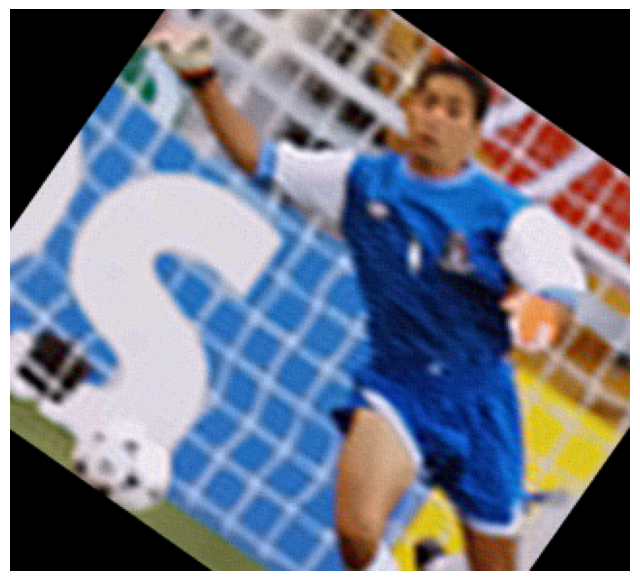
\includegraphics[width=0.45\textwidth]{images/Rotated Image.png}
    \caption{Rotación}
    \label{fig:img7}
\end{figure}

\section{Discusión}
El proceso de mejora de la imagen a través de la combinación de varios filtros y técnicas permitió alcanzar los objetivos de manera efectiva. Uno de los mayores retos fue equilibrar la eliminación de ruido con la preservación de detalles, pero el uso combinado de los filtros Sharpened, Non-local Means y Fourier proporcionó buenos resultados. La rotación final y el recorte aseguraron que el resultado final cumpliera con las especificaciones del examen.

\section{Conclusión}
El proceso de mejorar una imagen con ruido y desenfoque utilizando OpenCV y técnicas de procesamiento de imágenes como convolución y transformada de Fourier fue satisfactorio. Los resultados muestran que es posible mejorar notablemente la calidad visual de una imagen a través de una adecuada combinación de filtros.
\small
\bibliographystyle{plain}
\bibliography{ref}
\end{document}
